\PassOptionsToPackage{dvipsnames,table}{xcolor}
\documentclass[10pt]{beamer}
\usepackage{Cours}

\begin{document}

\input{\detokenize{/home/fenarius/Travail/Cours/NSITerminale/docs/commun/MacrosCours.tex}}
\setcounter{numchap}{4}

\newcommand{\DR}{\cnum Diviser pour régner}

\pythonmode



\begin{frame}
	\mframe{\DR}
	\begin{block}{\textcolor{yellow}{\rappel} Notion de complexité d'un algorithme}
		Lorsqu'on s'intéresse aux performances d'un algorithme, on fait varier le volume de données traité par l'algorithme et on étudie :
		\begin{itemize}
			\item<2-> l'évolution du nombre d'opération nécessaires au fonctionnement de l'algorithme, c'est ce qu'on appelle la \textcolor{red}{la compléxité en temps} de l'algorithme.
			\item<3-> l'évolution de l'espace mémoire nécessaire au fonctionnement de l'algorithme, c'est ce qu'on appelle la \textcolor{red}{la compléxité spatiale} de l'algorithme.
		\end{itemize}
	\end{block}
\end{frame}

\begin{frame}
	\mframe{\DR}
	\begin{block}{Complexité linéaire}
		\begin{itemize}
			\item<2-> On dira qu'un algorithme a une complexité en temps \textcolor{red}{linéaire} lorsque qu'un multiplication de la taille des données par un facteur $k$ se traduit par une augmentation du temps de calcul par un facteur proche de $k$.
			\item<3-> Par exemple si la complexité est linéaire traiter une liste \textcolor{red}{10} fois plus grande prendra environ \textcolor{red}{10} fois plus de temps
			\item<4-> Dans ce cas lorsqu'on trace le graphique du temps de calcul en fonction de la taille des données on obtient une \textcolor{red}{droite}.
		\end{itemize}
	\end{block}
	\onslide<5->{
		\begin{exampleblock}{Exemple}
			Un algorithme de parcourt simple d'une liste (par exemple recherche de minimum ou calcul de moyenne) a une complexité linéaire.
		\end{exampleblock}}
\end{frame}

\begin{frame}
	\mframe{\DR}
	\begin{block}{Complexité quadratique}
		\begin{itemize}
			\item<2-> On dira qu'un algorithme a une complexité en temps \textcolor{red}{quadratique} lorsque qu'un multiplication de la taille des données par un facteur $k$ se traduit par une augmentation du temps de calcul par un facteur proche de $k^2$.
			\item<3-> Par exemple si la complexité est quadratique traiter une liste \textcolor{red}{10} fois plus grande prendra environ \textcolor{red}{100} fois plus de temps
			\item<4-> Dans ce cas lorsqu'on trace le graphique du temps de calcul en fonction de la taille des données on obtient une \textcolor{red}{parabole}.
		\end{itemize}
	\end{block}
	\onslide<5->{
		\begin{exampleblock}{Exemple}
			Les algorithmes de tri par insertion ou par sélection ont une complexité quadratique.
		\end{exampleblock}}
\end{frame}

\begin{frame}
	\mframe{\DR}
	\begin{alertblock}{A retenir !}
		\begin{tabularx}{\textwidth}{|c|p{4cm}|X|}
            \hline
            Complexité & Nom & Exemple \\
            \hline
            $O(1)$ & Temps constant & Accéder à un élément d'une liste \\
            \hline
            $O(\log(n))$ & Complexité logarithmique & Recherche dichotomique dans une liste \\
			\hline
            $O(n)$ & Complexité linéaire & Recherche simple dans une liste \\
            \hline
            $O(n^2)$ & Complexité quadratique & Tri par insertion d'une liste \\
            \hline
            $O(2^n)$ & Complexité exponentielle & Algorithme par force brute pour le sac à dos \\
            \hline
		\end{tabularx}
	\end{alertblock}
\end{frame}

\begin{frame}
	\mframe{\DR}
	\begin{block}{Représentation graphique}
        \begin{center}
		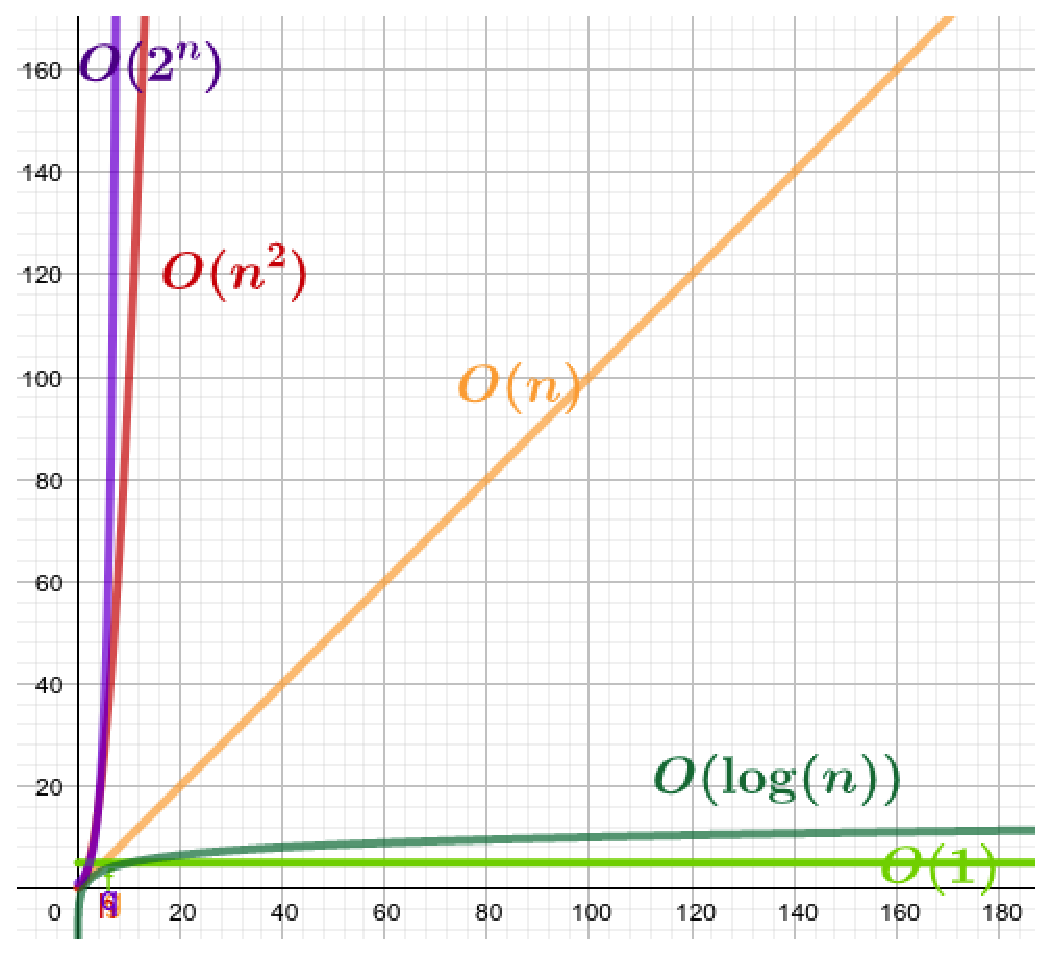
\includegraphics[scale=0.4]{complexite.eps}
        \end{center}
	\end{block}
\end{frame}


\begin{frame}
	\mframe{\DR}
	\begin{exampleblock}{Exemples}
		\begin{itemize}
			\item<1-> On suppose qu'on dispose d'un algorithme de complexité linéaire travaillant sur une liste, il traite une liste de \numprint{1000} éléments en \numprint{0.015} secondes. Donner une estimation du temps de calcul pour une liste de \numprint{250000} éléments.\\
			      \onslide<2-> {\textcolor{OliveGreen}{La taille des données a été multiplié par 250, la complexité étant lineaire le temps de calcul sera aussi approximativement multiplié par 250. \\}}
			      \onslide<3->{\textcolor{OliveGreen}{$0.015 \times 250 = 3.75$, on peut donc prévoir un temps de calcul d'environ 3,75 secondes}}
			\item<4-> Même question pour un algorithme de complexité quadratique qui traite une liste de \numprint{1000} éléments en \numprint{0.07} secondes.\\
			      \onslide<5-> {\textcolor{OliveGreen}{La taille des données a été multiplié par 250, la complexité étant quadratique le temps de calcul sera  approximativement multiplié par $250^2=62500$ \\}}
			      \onslide<6->{\textcolor{OliveGreen}{$0.07 \times 62\,500 = 4375$, on peut donc prévoir un temps de calcul d'environ $4\,375$ secondes, c'est à dire près d'une heure et 15 minutes !}}
		\end{itemize}
	\end{exampleblock}
\end{frame}


\begin{frame}
	\mframe{\DR}
	\begin{alertblock}{Principe de la méthode}
		La méthode \textcolor{red}{diviser pour régner} (en anglais \textit{divide and conquer})  est une technique algorithmique qui consiste à :        \begin{enumerate}
			\item<2-> décomposer le problème initial en un ou plusieurs sous problèmes de taille inférieure,
			\item<3-> résoudre chacun des sous problèmes,
			\item<4-> combiner les solutions des sous problèmes pour obtenir la solution au problème initial.
		\end{enumerate}
	\end{alertblock}
	\onslide<5->{
		\begin{exampleblock}{Exemple}
			L'algorithme de \textcolor{blue}{recherche dichotomique} dans un tableau \textbf{trié} déjà rencontré en classe de première est un exemple de la méthode diviser pour régner.
			Le sous problème est alors la recherche dans une liste de taille deux fois plus petite.
		\end{exampleblock}}
\end{frame}

\begin{frame}
	\mframe{\DR}
	\begin{alertblock}{Tri fusion}
		L'algorithme du \textcolor{red}{tri fusion} (en anglais \textit{merge sort})  illustre parfaitement la méthode diviser pour régner, en effet, il consiste à
		\begin{enumerate}
			\item<2-> Décomposer la liste en deux sous listes de longueur égale (à une unité près).
			\item<3-> Trier chacune des sous listes (c'est donc un algorithme récursif)
			\item<4-> Fusionner les parties triées
		\end{enumerate}
	\end{alertblock}
\end{frame}


\begin{frame}
	\mframe{\DR}
	\begin{exampleblock}{Exemples}
		Pour illuster la méthode diviser pour régner, on peut aussi citer :
		\begin{itemize}
			\item<2-> La tri rapide (en anglais \textit{quicksort}),
			\item<3-> Le quart de tour d'une image,
			\item<4-> La recherche des deux points les plus proches,
			\item<5-> L'algorithme de multiplication rapide de Karatsuba.
		\end{itemize}
	\end{exampleblock}
\end{frame}

\end{document}